%%%%%%%%%%%%%%%%%%%%%%%%%%%%%%%%%%%%%%%%%
% University/School Laboratory Report
% LaTeX Template
% Version 3.0 (4/2/13)
%
% This template has been downloaded from:
% http://www.LaTeXTemplates.com
%
% Original author:
% Linux and Unix Users Group at Virginia Tech Wiki
% (https://vtluug.org/wiki/Example_LaTeX_chem_lab_report)
%
% License:
% CC BY-NC-SA 3.0 (http://creativecommons.org/licenses/by-nc-sa/3.0/)
%
%%%%%%%%%%%%%%%%%%%%%%%%%%%%%%%%%%%%%%%%%

%----------------------------------------------------------------------------------------
%	PACKAGES AND DOCUMENT CONFIGURATIONS
%----------------------------------------------------------------------------------------

\documentclass{article}

\usepackage{mhchem} % Package for chemical equation typesetting
\usepackage{siunitx} % Provides the \SI{}{} command for typesetting SI units
\usepackage{hyperref}
\usepackage{graphicx} % Required for the inclusion of images
\usepackage{tabularx}
\usepackage{float}
\usepackage{algorithm}
\usepackage{algpseudocode}
\usepackage{bm}
\usepackage{multirow}% http://ctan.org/pkg/multirow
\usepackage{hhline}% http://ctan.org/pkg/hhline
\usepackage{caption}
\usepackage{subcaption}
\usepackage{listings}
\usepackage{xcolor}
\usepackage[letterpaper, margin=0.9in]{geometry}
\lstset{
    %numbers=left,
    stepnumber=1,    
    firstnumber=1,
    numberfirstline=true,
    basicstyle=\ttfamily,
    keywordstyle=\color{blue}\ttfamily,
    stringstyle=\color{red}\ttfamily,
    commentstyle=\color{green}\ttfamily,
    breaklines=true,
}


\setlength\parindent{0pt} % Removes all indentation from paragraphs

\renewcommand{\labelenumi}{\alph{enumi}.} % Make numbering in the enumerate
% environment by letter rather than number (e.g. section 6)

%\usepackage{times} % Uncomment to use the Times New Roman font

%----------------------------------------------------------------------------------------
%	DOCUMENT INFORMATION
%----------------------------------------------------------------------------------------

\title{UC Davis STA 208 2016 Spring Midterm Exam} %
% Title
\author{Wenhao \textsc{Wu}, 998587583} % Author name
\date{\today} % Date for the report

\begin{document}
\maketitle % Insert the title, author and date

% If you wish to include an abstract, uncomment the lines below

\section{Data Description}
This dataset contains $N=3089$ observations of $p=4$ features. Among this
observations $N_0=1089$ observations are labeled with the response $y=0$ and
$N_1= 2000$ observations with $y=1$, and the formers are located in the second
half of the data file while the latter in the first half.
The scatterplot matrix of the dataset is shown in Fig.~\ref{fig:scatterplot}
\begin{figure}[h]
  \centering
  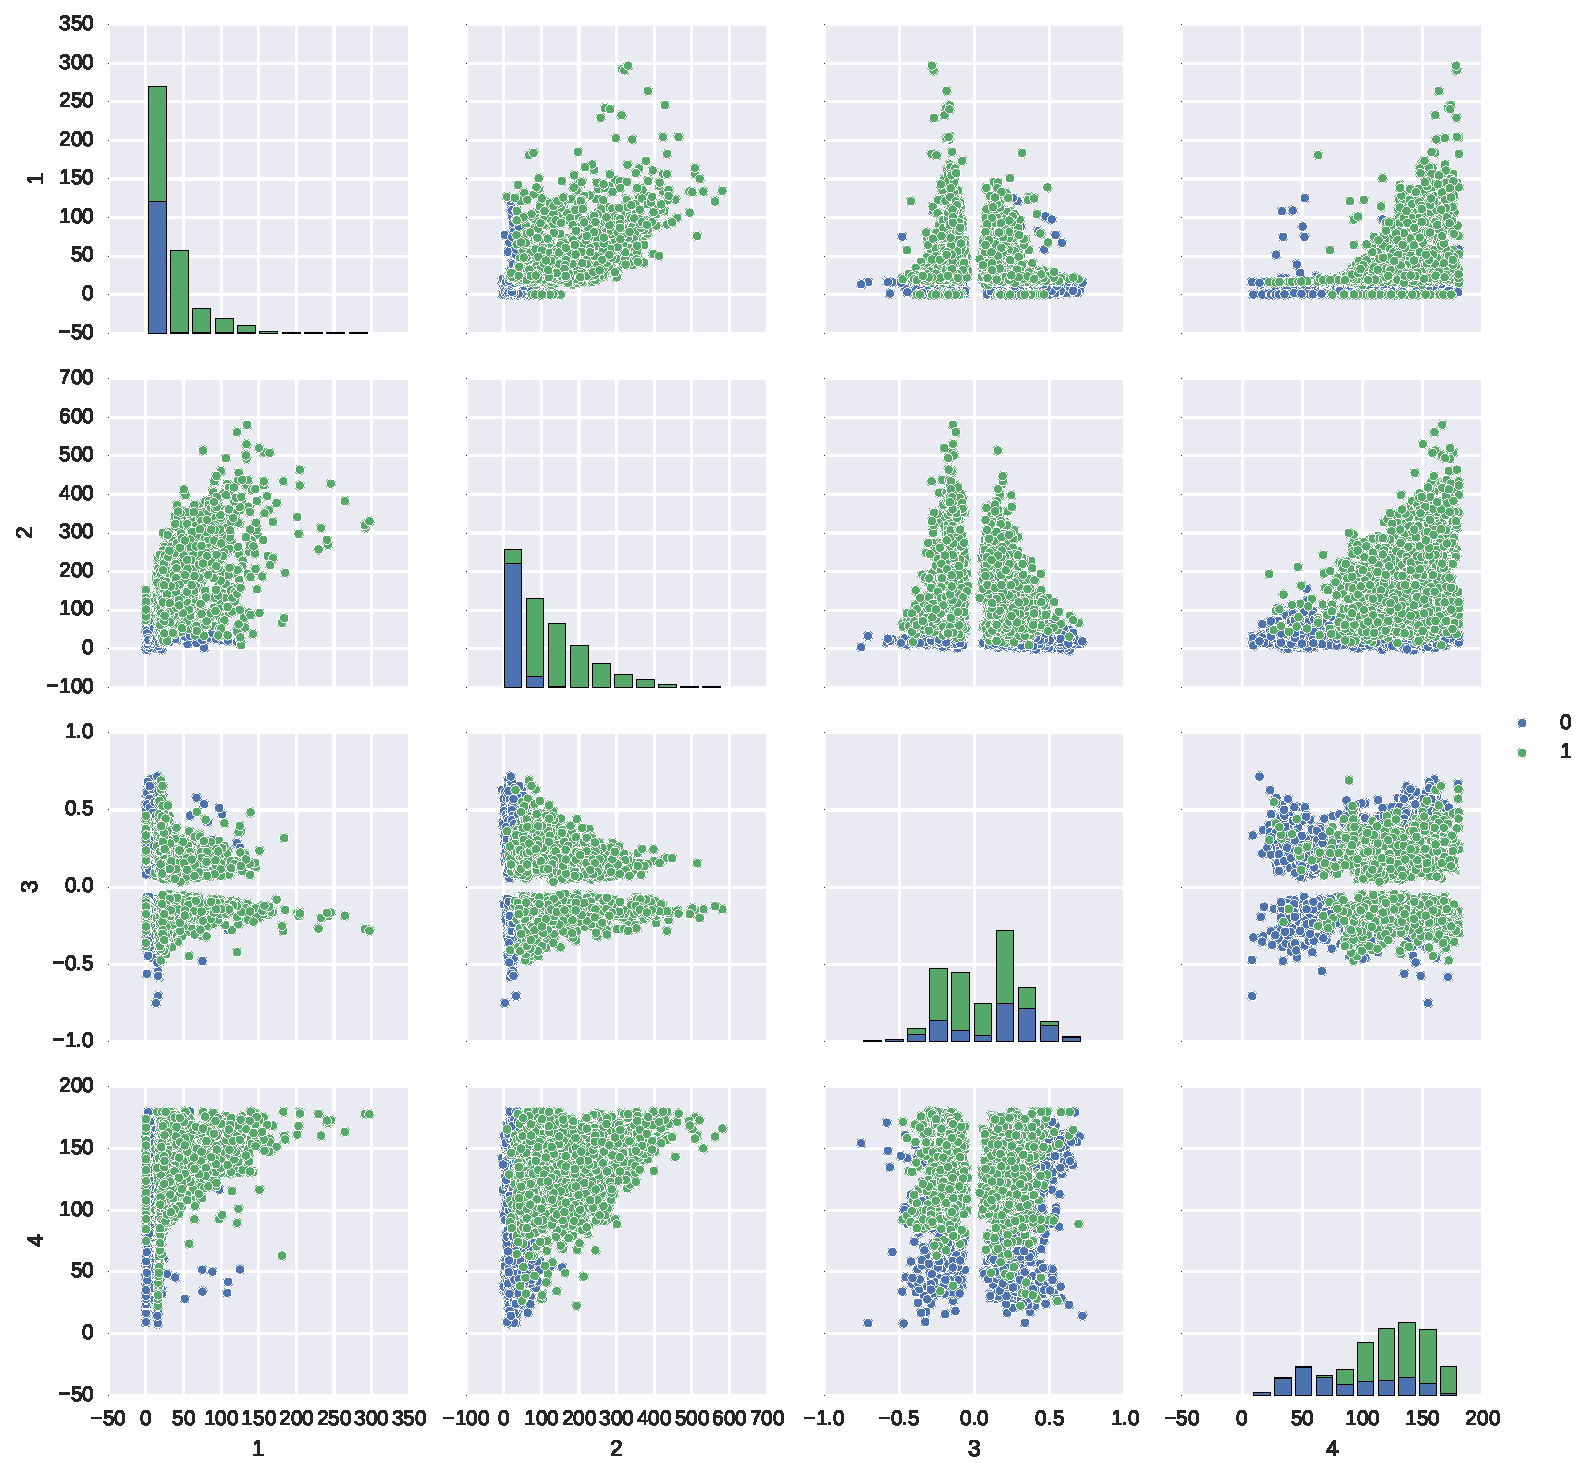
\includegraphics[width=0.8\textwidth]{figs/scatterplot.pdf}
  \caption{The scatterplot matrix of the dataset.}
  \label{fig:scatterplot}
\end{figure}

\section{Algorithm Design}
In order to train and test our classifier, firstly we set aside $\%25$ of the
observation as a testing set. The parameters of our classifiers are tuned
using 10-fold cross-validation using the rest $\%75$ observations.
Prior to the training, the data is preprocessed so that each feature has zero
mean and unit variance.

Since the dimension of the input variables is rather low and the number of
observations is relatively small, we first try to tune a simple
$k$-Nearest-Neighbor (KNN) classifier on the 4 given features. The results are
shown in Fig.~\ref{fig:knn_tune}. The 10-fold cross validation suggests that
when $k\in[3, 30]$ the validation score is maximized, where the KNN classifier 
results in a decent test score of $\sim0.95$. We select $k=15$ for our KNN
classifier.

\begin{figure}[h]
  \centering
  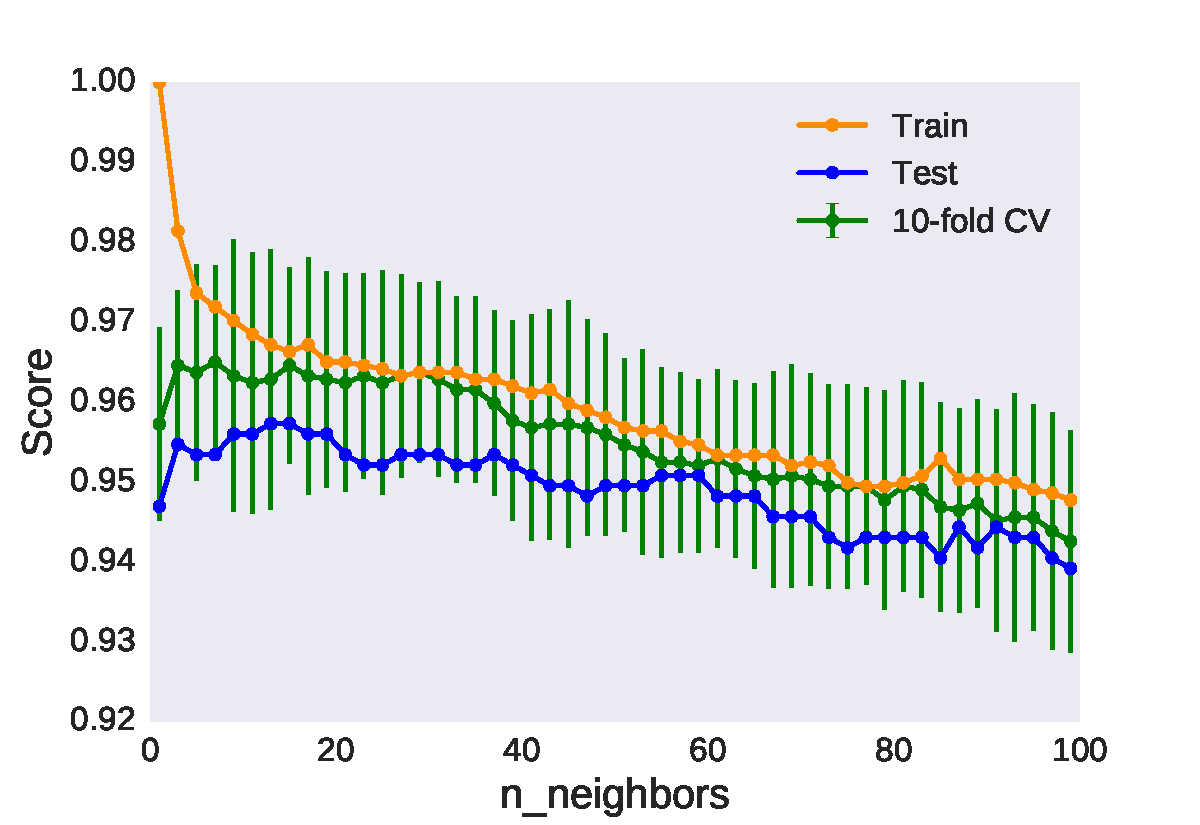
\includegraphics[width=0.5\textwidth]{figs/knn_tuning.pdf}
  \caption{Tuning the KNN classifier.}
  \label{fig:knn_tune}
\end{figure}

Although KNN results in a decent performance accuracy, we would like to try
other machine learning methods with better interpretability. Here we tried
decision tree model in which the depth of the tree is tuned with
cross-validation. The results is shown in Fig.~\ref{fig:tree_tune}. It appears
that the cross-validation favors a depth of 3 which also results in a test score
of $\sim0.95$, for which the decision tree fitted on the training set is shown
in Fig.~\ref{fig:tree_structure}.

\begin{figure}[h]
  \centering
  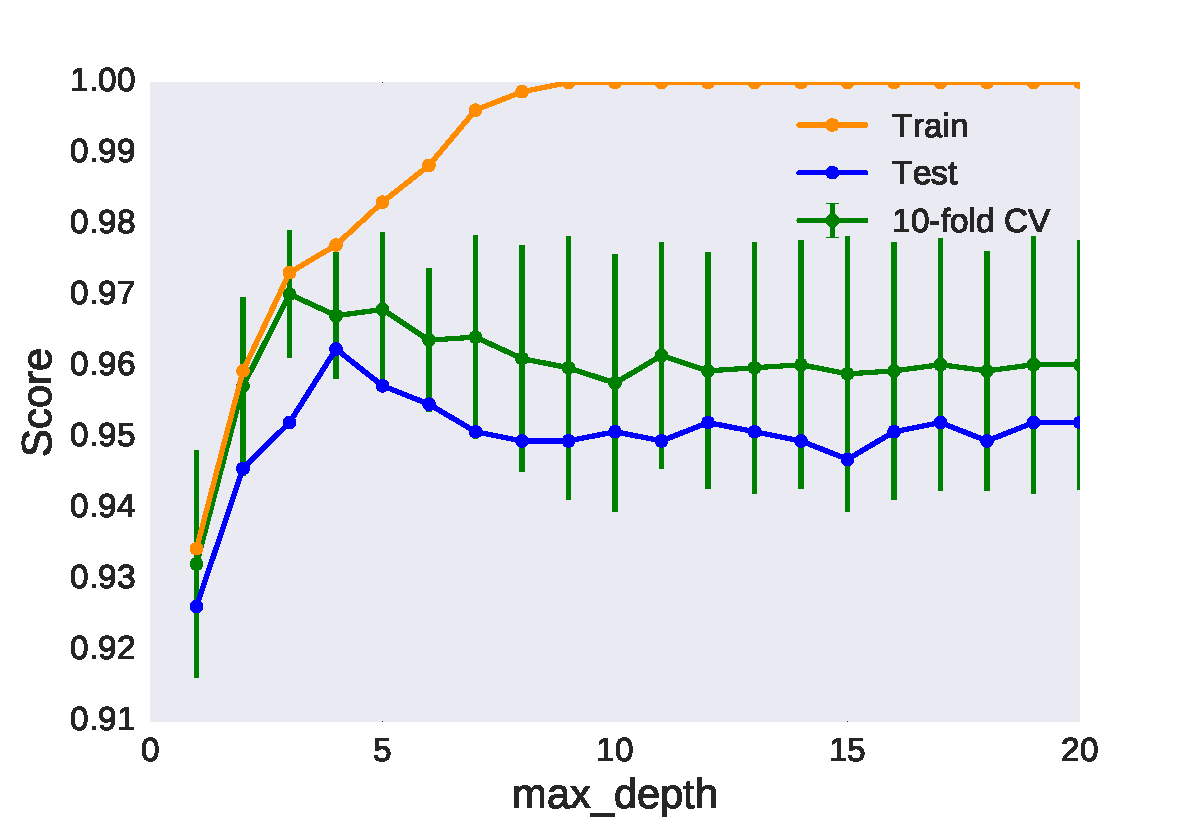
\includegraphics[width=0.5\textwidth]{figs/tree_tuning.pdf}
  \caption{Tuning the decision tree classifier.}
  \label{fig:tree_tune}
\end{figure}

\begin{figure}[h]
  \centering
  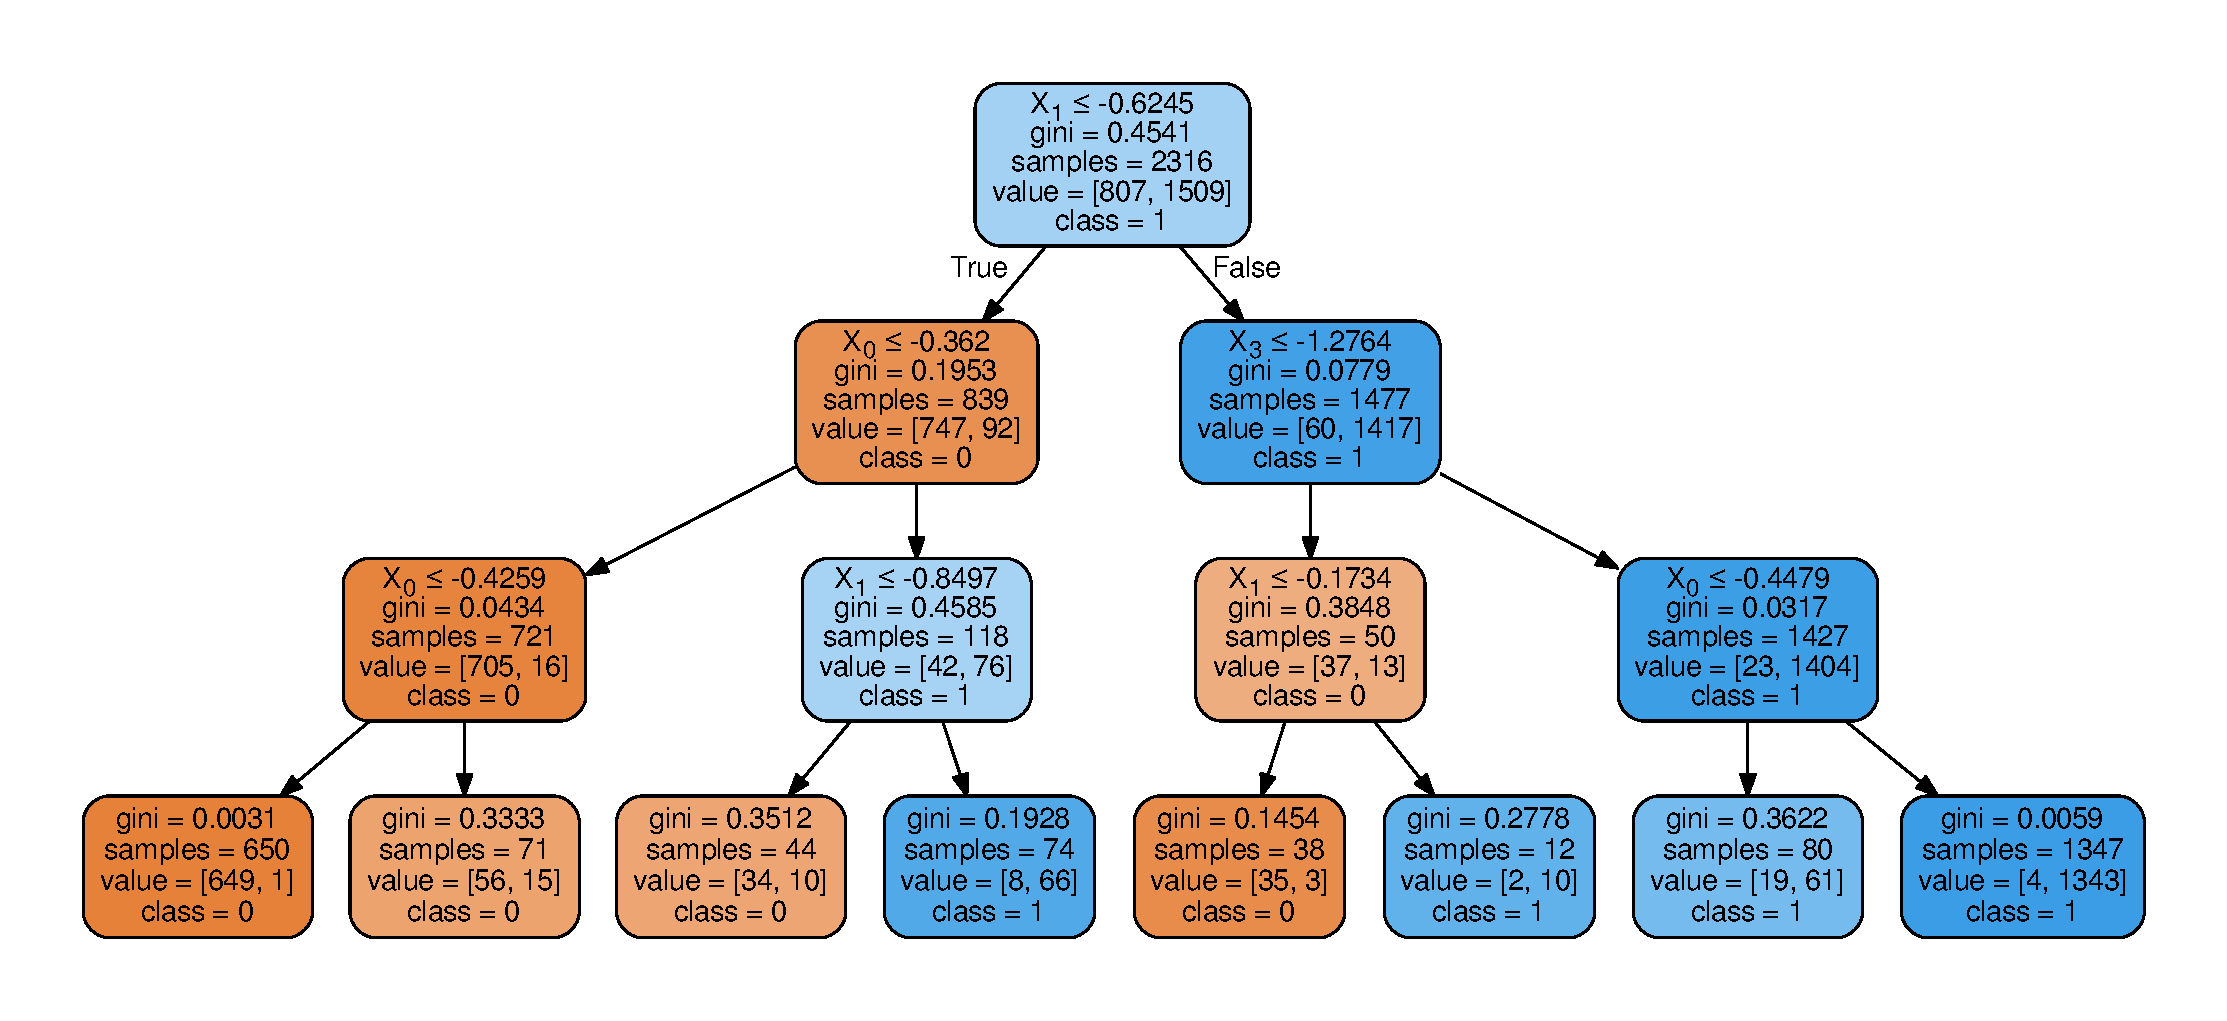
\includegraphics[width=0.9\textwidth]{figs/tree_structure.pdf}
  \caption{The trained decision tree classifier.}
  \label{fig:tree_structure}
\end{figure}

\section{Numerical Results and Conclusion}



%   BIBLIOGRAPHY
%----------------------------------------------------------------------------------------

%\bibliographystyle{unsrt}
%\bibliography{myrefs}

%\pagebreak


%----------------------------------------------------------------------------------------


\end{document}